\documentclass{article}
%\usepackage[latin1]{inputenc}
\usepackage{graphicx,amssymb,amsmath,amsbsy} % extensions pour maths avancées
\usepackage{graphicx}           % extensions pour figures
\usepackage[T1]{fontenc}        % pour les charactères accentués 
\usepackage[utf8]{inputenc} 

\usepackage{stmaryrd} % Pour les crochets d'ensemble d'entier

\DeclareMathOperator{\tr}{tr}
\DeclareMathOperator{\argmax}{argmax}


\setlength{\parindent}{0.0in}
\setlength{\parskip}{0.3in}
\setlength{\topmargin}{-0.4in}
\setlength{\topskip}{1in}    % between header and text
\setlength{\textheight}{8in} % height of main text
\setlength{\textwidth}{4.5in}    % width of text
\setlength{\oddsidemargin}{1in} % odd page left margin
\setlength{\evensidemargin}{1in} % even page left margin
%
%% Quelques raccourcis clavier :
\def\slantfrac#1#2{\kern.1em^{#1}\kern-.3em/\kern-.1em_{#2}}
\def\b#1{\mathbf{#1}}
\def\bs#1{\boldsymbol{#1}}
\def\m#1{\mathrm{#1}}
%
\newcommand{\greeksym}[1]{{\usefont{U}{psy}{m}{n}#1}}
\newcommand{\inc}{\mbox{\small\greeksym{d}\hskip 0.05ex}}%
\pagenumbering{arabic}
\date{\today}
\title{Modèles Graphiques}
\author{Barbara Gris \& Nelle Varoquaux}
\begin{document}
\maketitle
\tableofcontents{}
\vfill \eject


\section{Apprentissage dans les modèles discrets}

Soit $z$ et $x$ deux variables aléatoires pouvant prendre
respectivement $N$ et $K$ valeurs telles que: $p(z= m) =
\pi_m$ et $p(x=k|z=m) = \theta_{mk}$

On suppose que l'on observe $n$ valeurs $(x_i, z_i)$ iid. On note 
$N_{i, j}$ le cardinal de 
$\{k \in \llbracket 1, n \rrbracket | (x_{k}, z_k = (i, j))\}$ et $N_i$ celui
de $\{j \in \llbracket 1, n \rrbracket | (z_j = i )\}$.

L'estimateur $(\pi, \theta)$ du maximum de vraisemblance est:

$(\pi, \theta) = \argmax \prod_{i=1}^n p(x_i, z_i)$

$(\pi, \theta) = \argmax \prod_{i=1}^n \prod_{j=1}^K \pi_i^{N_ij} \theta_{i,j}^{N_{ij}}$

$(\pi, \theta) = \argmax \sum_{i=1}^{m} \sum_{j=1}^k n_{ij}(log\pi_{ij} + \log(\theta_{ij})$

$(\pi, \theta) = \argmax \sum_{i=1}^{m} \sum_{j=1}^k n_{ij}log\pi_{ij} + \sum_{i=1}^{m} \sum_{j=1}^k n_{ij}\log(\theta_{ij}$

$(\pi, \theta) = \argmax \sum_{i=1}^{m} \sum_{j=1}^k n_{ij}log\pi_{ij} + \sum_{i=1}^{m} \sum_{j=1}^k n_{ij}\log(\theta_{ij}$

On a donc:
$$\pi = \argmax \sum_{i=1}^{M} \sum_{j=1}^K N_{ij} log\pi_i$$
$$\theta = (\theta_1, ... \theta_M)$$

avec $\theta_i = \argmax \sum_{k=i}^M \pi_k - 1$


Contraintes:

$\sum_{i = 1}^M \pi_m = 1$
$\forall 0 < i < M, \pi_i > 0$

$\forall m | 1 \leq m \leq M, \sum_{k = 1}^K \theta_{mk} = 1, \theta_{mk}
> 0$

\subsection{Calcul du maximum de vraisemblance de $\pi$}

$p_\pi(\delta^{(1)}, .. \delta^{^(n)}) = \prod_{i=1}^n p (\delta_{i} | \pi)$

Or les variables sont iid:

$p_\pi(\delta^{(1)}, .. \delta^{^(n)}) = \prod_{i=1}^n \pi_1^{\delta_1^{(i)}},
.., \pi_k^{\delta_k^{(i)}}$

$l(\pi) = \log(p(\delta^{(1)}, .. \delta^{(n)}[\theta)$

$l(\pi) = \sum_{i=1}^n log(\prod_{k=1}^K \pi_k^{\delta_k(i)})$

$l(\pi) = \sum_{i=1}^n \sum_{k=1}^K log(\pi_k^{\delta_k(i)})$

En utilisant la méthode des Lagrangiens,

$\mathcal{L}(\pi, \lambda) = \sum_{i, k} \delta_k^{(i)} log \pi_k +
\lambda(\sum_{k=1}^K \pi_k - 1)$

$\max_\theta \min_{\lambda \in \mathbb{R}} \mathcal{L}(\theta, \lambda) =
\min_\theta \max_{\lambda \in \mathbb{R}} \mathcal{L}(\theta, \lambda)$

$\frac{\partial \mathcal{L}(\theta, \lambda}{\partial \pi_j} = \sum_{i=1}^n
\frac{\delta_j^{(i)}}{\pi_j} + \lambda$

Donc

$$\pi_j = \frac{-N_j}{\lambda}$$

avec $N_j = \#\{ i | x_i = j \} = \#\{ i | \delta_j^{(i)} = 1 \}$

En utilisant les contraintes, on en déduit :

$\sum_{i=j}^K \pi_i = 1 = \sum_{i=1}^K \frac{- N_k}{\lambda}$

\subsection{Maximum de Vraisemblance de $\theta$}


On a $p(x=k|z=m)= \theta_{mk}$.

De même que précédement, on a:

$$\theta_{mk} = \frac{N_{mk}}{n}$$

avec $N_{mk} = \#\{k|\delta_j^{(k)} = 1 | z = m\}$

\section{Classification linéaire}

\subsection{Modèle LDA}
A REDIGER

$l(\theta) = log(\prod_{n=1}^N p (y_n | \pi) \prod_{j=1}^m p(x_{j, n}|y_n, \theta_j)$

$l(\theta) = \sum_{n=1}^N \log(p(y_n |\pi) + \sum_{n=1}^{N}\sum_{j=1}^m \log(p(x_{j, n}|y_n, \theta_j))$

On peut donc maximiser le premier terme indépendemant du deuxième terme.

D'après l'exercice 1, $\pi_{MV} = \frac{\sum_{i=1}^N y_i}{N}$

Le deuxième terme s'écrit:

$l_2(\theta) = \sum_{n=1}^N \sum_{j=1}^m
\log((\frac{1}{(2\pi)^{m/2}|\Sigma|^{1/2}}\exp(\frac{-1}{2}(x-\mu_j)^{T}\Sigma^{-1}(x-\mu_j))^{y_n}))$

Or $m =2$

% Donc, $\forall i \in \llbracket0, m \rrbracket$
%
% $\mu_{j, MV} = argmax \{\sum_{n=1}^N
% \log[\frac{1}{(2\pi)^{d/2}|\Sigma|^{1/2}}\exp(\frac{-1}{2}(x-\mu_j)^T\Sigma^{-1}(x-\mu_j))]\}$

$l_2(\theta) = -n(\log(2\pi|\Sigma|^{1/2})) - \frac{1}{2}\sum_{j=1}^{n}y_j(x_j - \mu_1)^T\Sigma^{-1}(x_j - \mu_1)
- \frac{1}{2}\sum_{j=1}^{n}(1 - y_j)(x_j - \mu_0)^T\Sigma^{-1}(x_j - \mu_0)$


$l_2(\theta) = -n(\log(2\pi|\Sigma|^{1/2})) - \frac{1}{2}\sum_{j=1}^{n} y_j \tr(\Sigma^{-1} (x_i - \mu_1)(x_i - \mu_1)^T - \frac{1}{2}\sum_{j=1}^{n} (1 - y_j)\tr(\Sigma^{-1} (x_i - \mu_0)(x_i - \mu_0)^T$

$l_2(\theta)$ est donc composé de trois termes:

\begin{equation}
a = -n(\log(2\pi|\Sigma|^{1/2}))
\end{equation}

\begin{equation}
b = - \frac{1}{2}\sum_{j=1}^{n} y_j \tr(\Sigma^{-1} (x_i - \mu_1)(x_i - \mu_1)^T
\end{equation}


\begin{equation}
c = - \frac{1}{2}\sum_{j=1}^{n} (1 - y_j)\tr(\Sigma^{-1} (x_i - \mu_0)(x_i - \mu_0)^T
\end{equation}

DEMONSTRATION A FINIR

$\mu_1 = \frac{1}{n} \sum_{i=1}^{N_j}x_i$

\subsection{Comparaison des trois modèles}


\begin{tabular}{| c | l | l | l |}
          & LDA & Régression Logistique & Régression Linéaire \\
A         & 0.216667 & \textbf{0.16}    & \textbf{0.16}      \\
B         & 0.126667 & 0.1     & \textbf{0.08333}   \\
C         & 0.155    & \textbf{0.12}    & 0.16       \\
\end{tabular}


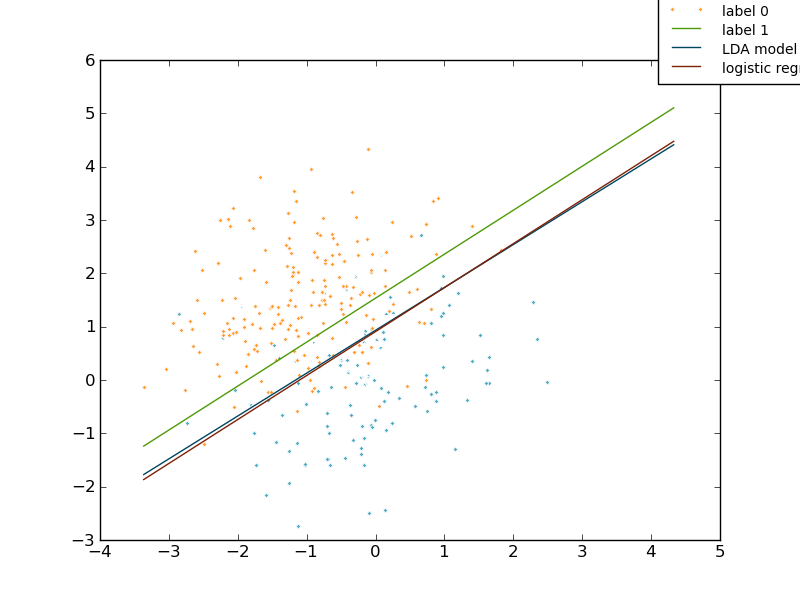
\includegraphics[width=300px]{classificationA1.png}


\paragraph{Jeu de données A}

Le barycentre des données est équidistant des nuages de points $Y = 0$ et $Y =
1$, ce qui explique la bonne performance de la régression linéaire.

Entre LDA et IRLS, la pente des droites est très proche, mais la constante
varie. IRLS est une méthode d'approximation itérative, qui suit le même
principe que LMS (least mean square), qui converge très bien pour la
régression linéaire. Comme cette dernière est très efficace ici, il n'est donc
pas surprenant qu'IRLS marche si bien sur ces données.

On peut supposer que si il y a un biais dans les données, il sera plus
facilement corrigé par un algorithme itératif (IRLS) que par un calcul direct
(LDA). Cela peut expliquer le plus faible taux d'erreur pour IRLS que pour
LDA.


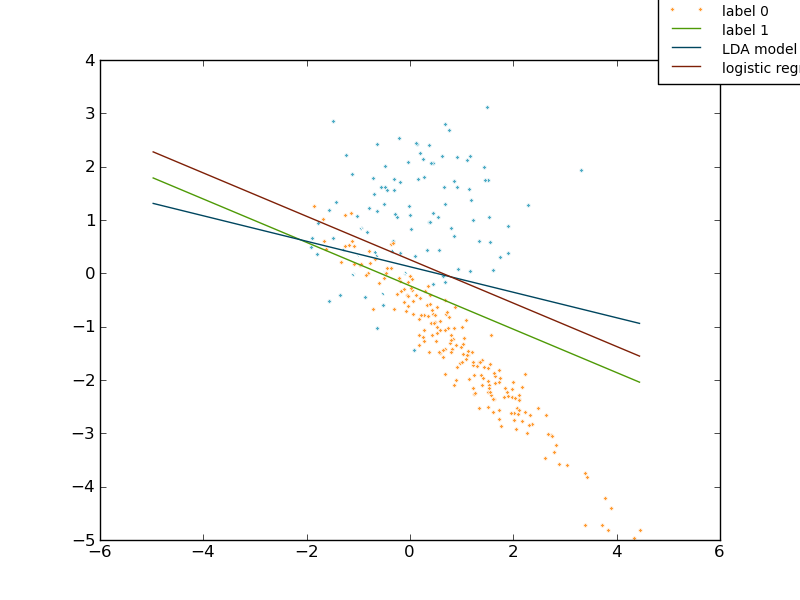
\includegraphics[width=300px]{classificationB1.png}


\paragraph{Jeu de tests B}

La régression linéaire fonctionne très bien sur ce jeu de données, car les
points tels que $Y = 1$ sont visuellement proches d'une droite, qui est elle
même orthogonal à la moyenne des vecteurs pour $Y = 0$. Ainsi il semble
réaliste de trouver un vecteur $\theta$ tel que pour le point X tel que $Y = 1$,
$\theta X = 1$, et dans l'autre cas $\theta X = 0$

On remarque que les deux autres méthodes sont aussi relativement bonnes. Ce
n'est pas surprenant, les données étant visuellement séparées.

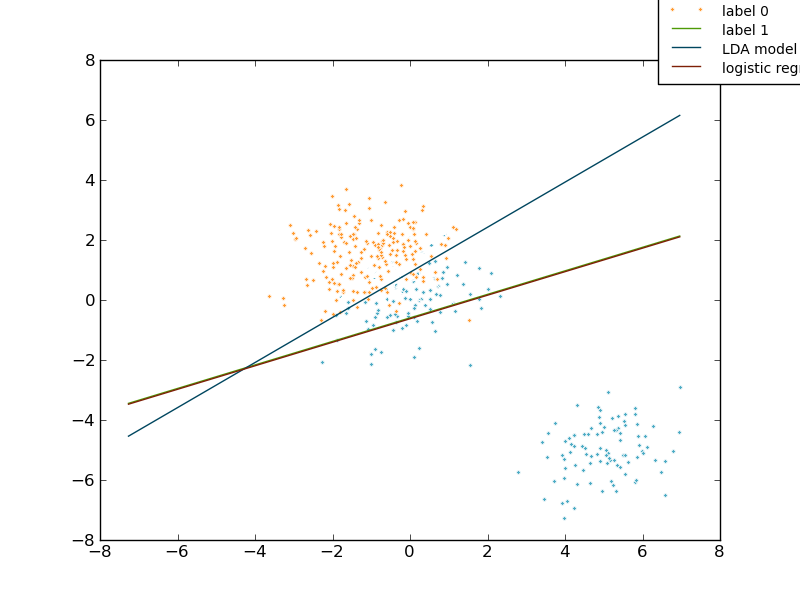
\includegraphics[width=300px]{classificationC1.png}


\paragraph{Jeu de tests C}

Les points sont visuellement proche d'une même droite. Si un vecteur $\theta$
est tel que $\theta X = 1$ pour $Y = 1$, alors pour une grande partie des
points tels que $Y = 0$, on aura aussi $\theta X = 1$. Pour la régression
linéaire, la distance au barycentre des points joue énormement (mauvais
traitement des données bimodales). Même les points exceptionnellement éloignés
du barycentre ont une importance sur le calcul de theta, alors qu'ils
représentent plus du bruit. La régression linéaire est très peu robuste.

De même que pour le jeu de données B, IRLS et LDA donnent des résultats tout à
fait satisfaisants.


\end{document}
